
\chapter{Sintesi a Campionamento}


\section{Principi di Base}

\begin{itemize}
    \item Il teorema del campionamento garantisce che qualsiasi segnale campionato secondo il teorema di Nyquist può essere perfettamente memorizzato e richiamato per la riproduzione e la conversione D/A.
    \item PCM (Pulse Code Modulation): tecnica usata nei CD audio (16 bit, 44100 Hz).
\end{itemize}
\begin{figure}[H]
    \centering
    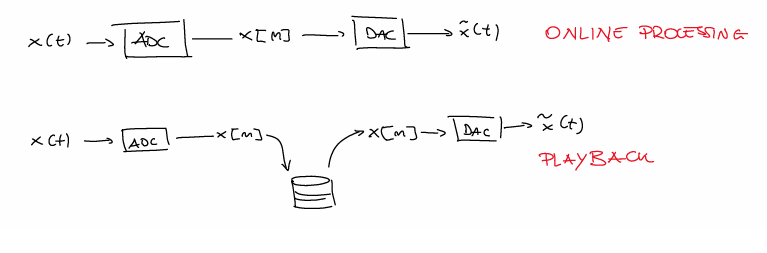
\includegraphics[width=0.7\textwidth]{capitoli/capitolo13/immagini/image1.png}
\end{figure}

\section{Sintesi a Campionamento}

\begin{itemize}
    \item Registrazione, memorizzazione e riproduzione di frammenti sonori.
    \item Adatta per strumenti musicali, voce e suoni complessi.
    \item Non è possibile campionare ogni possibile suono, perciò si rende necessaria una discretizzazione.
\end{itemize}

\section{Esempi: Sintesi a Campionamento}

\subsection{Violino}

\begin{itemize}
    \item \textbf{Pitch}: qualsiasi valore reale nell'intervallo 196--3136 Hz.
    \item \textbf{Forza dell'archetto}: a partire dal valore minimo che produce un tono sostenuto (non un suono stridente).
    \item \textbf{Durata}: da una frazione di secondo a ore.
\end{itemize}

\subsection{Pianoforte}

\begin{itemize}
    \item \textbf{Pitch}: 88 tasti.
    \item \textbf{Velocity}: da pianissimo a fortissimo (approssimativamente da 1 a 50 N).
    \item \textbf{Durata}: da pochi millisecondi a diversi secondi.
\end{itemize}

\noindent
\textit{È impossibile registrare un numero infinito di suoni!}

\section{Discretizzazione dei Dati}

\begin{itemize}
    \item È possibile trovare un modo efficace per discretizzare tutti questi dati.
    \item \textbf{JND (Just Noticeable Difference)} per l'altezza:
    \begin{itemize}
        \item Sotto i 500 Hz: circa 3 Hz per onde sinusoidali, 1 Hz per toni complessi.
        \item Sopra i 1000 Hz: circa 0.6\% per onde sinusoidali (circa 10 cents).
    \end{itemize}
    \item \textbf{Velocity}: piccole variazioni di forza non alterano significativamente il timbro.
    \item \textbf{Durata}: non definita in termini di JND, ma può essere discretizzata in base al contesto.
\end{itemize}

\section{Problemi Aggiuntivi}

\begin{itemize}
    \item \textbf{Pianoforte}: colpire un tasto con il sistema fermo produce un suono diverso rispetto a colpirlo mentre è ancora in vibrazione (ribattuto).
    \item \textbf{Violino}: la posizione dell'archetto sulla corda influisce sul timbro.
\end{itemize}

\noindent
\textit{È davvero impossibile registrare tutti questi suoni! Ma possiamo applicare i principi dell'elaborazione digitale del segnale per modificare pochi suoni registrati e ottenere una grande varietà di risultati.}

\section{Pitch}

\begin{itemize}
    \item Cosa succede se si legge un nastro a velocità diverse?
    \item Possiamo leggere i campioni memorizzati alla velocità desiderata tramite interpolazione.
\end{itemize}
\begin{figure}[H]
    \centering
    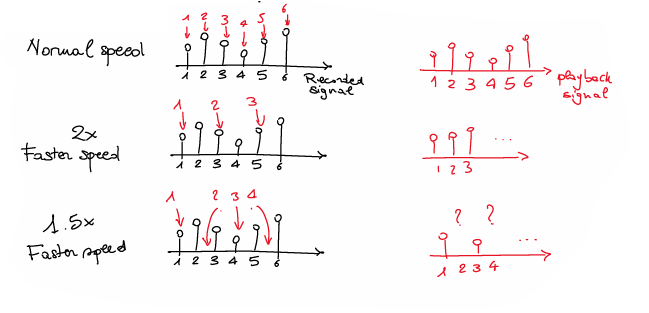
\includegraphics[width=0.7\textwidth]{capitoli/capitolo13/immagini/image2.png}
\end{figure}

\section{Il Problema delle Formanti}

\begin{itemize}
    \item Gli strumenti possono essere approssimati con un modello sorgente-filtro.
    \item Se si modifica l'intonazione variando la velocità di riproduzione, si modificano anche le formanti insieme alle armoniche.
    \item Negli strumenti reali devono cambiare solo le armoniche, non le formanti.
    \item Questo effetto è dovuto alla proprietà di time scaling di Fourier.
    \item Negli strumenti musicali reali siamo però più tolleranti ai cambiamenti di pitch.
\end{itemize}
\begin{figure}[H]
    \centering
    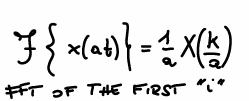
\includegraphics[width=0.3\textwidth]{capitoli/capitolo13/immagini/image3.jpeg}
\end{figure}

\section{Discretizzazione del Pitch}

\begin{itemize}
    \item Un solo tono non è sufficiente; cento sono troppi.
    \item Bisogna trovare un compromesso tra qualità e costi (dipende dall'applicazione e dall’hardware).
    \item Si può usare una discretizzazione approssimativa dell’intervallo di intonazione.
\end{itemize}

\section{Velocity (Intensità)}

\begin{itemize}
    \item È possibile usare un solo campione e modificare l’intensità via guadagno?
    \begin{itemize}
        \item A volte sì, ma raramente.
        \item Spesso non è sufficiente.
    \end{itemize}
    \item La discretizzazione può essere approssimativa:
    \begin{itemize}
        \item Esempio: Key velocity: 0, 30, 80, 127.
    \end{itemize}
    \item Problemi:
    \begin{itemize}
        \item L'aumento della forza può rendere udibili i passaggi di livello se la discretizzazione è troppo grossolana.
        \item Soluzione: somma di due segnali con guadagni complementari.
        \item Problemi della soluzione: costo computazionale doppio, richiede allineamento preciso di fase.
    \end{itemize}
    \item Esempio: Manuale d’uso AKAI S1100 (1990) – spiegazione delle velocity zones.
\end{itemize}

\section{Durata}

\begin{itemize}
    \item Per discretizzare la durata serve conoscere l’evoluzione temporale del segnale.
    \item Esempio: tono dell'organo a canne.
\end{itemize}

\section{Loops}

\begin{itemize}
    \item La scelta dei punti di inizio e fine del loop è molto importante.
\end{itemize}
\begin{figure}[H]
    \centering
    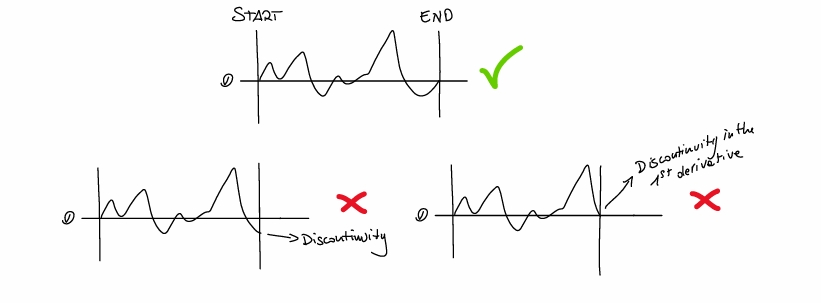
\includegraphics[width=0.7\textwidth]{capitoli/capitolo13/immagini/image4.jpeg}
\end{figure}


\section{Aspetti Tecnici}

\subsection{Costo Computazionale}

\begin{itemize}
    \item Interpolazione tra valori (es. lineare, spline).
    tabread4 = b+frac*\{ cminusb - 0.1666667f * (1.-frac)*[ (d - a - 3.0f * cminusb)*frac + (d + 
2.0f*a – 3.0f*b)]\}
    \item Calcolo di envelope (es. decadimento esponenziale).
    \item Compromesso tra qualità del suono e performance.
\end{itemize}

\subsection{Memoria}

\begin{itemize}
    \item I costi della RAM si sono notevolmente abbassati.
    \item I DSP moderni permettono l’utilizzo di campioni più complessi.
\end{itemize}

\section{Problemi e Limitazioni}

\begin{itemize}
    \item Gli algoritmi che mantengono invariate le formanti sono troppo costosi per l’uso in tempo reale.
    \item Layer dinamici complessi portano a una gestione difficile del timbro.
    \item Mancanza di espressività: tecniche come plettrata, palm mute, bending, ecc., sono difficili da riprodurre.
    \item Soluzioni: round robin (alternanza di campioni), maggiore layering e split, uso del protocollo MPE.
\end{itemize}

\section{Esempi di Sampler Hardware e Software}

\begin{itemize}
    \item AKAI S1100 (1990): 16 bit, 44.1 kHz, 2MB RAM espandibile.
    \item LEM Example (1988): 12 bit, 40.5 kHz.
    \item Elektron Digitakt (2017): 64MB RAM, 1GB storage.
    \item Dream SAM5916B: 16 DSP, 256 voci a 48kHz, decrypting on-the-fly.
\end{itemize}



